\documentclass[11pt]{article}
\usepackage{amsmath,amssymb,amsthm}
\usepackage{enumitem}
\usepackage{setspace}
\usepackage{xcolor}
\usepackage{graphicx}
\usepackage{geometry}
\usepackage{float}
\usepackage{titlesec}
\usepackage{subfigure}
\usepackage{caption}
\captionsetup{figurewithin=section}
\usepackage{amsmath}
\usepackage{enumitem}
\usepackage{amssymb}

\DeclareMathOperator*{\E}{\mathbb{E}}
\let\Pr\relax
\DeclareMathOperator*{\Pr}{\mathbb{P}}

\newcommand{\eps}{\varepsilon}
\newcommand{\inprod}[1]{\left\langle #1 \right\rangle}
\newcommand{\R}{\mathbb{R}}

\newcommand{\handout}[5]{
  \noindent
  \begin{center}
  \framebox{
    \vbox{
      \hbox to 5.78in { {\bf \centering ECE-GY 9243/ME-GY 7973} \hfill #2 } 
      \vspace{5mm} 
      \hbox to 5.78in { {\bf \Large Optimal and Learning Control for Robotics}}
      \vspace{4mm}
      \hbox to 5.78in { {\Large \hfill #5  \hfill} }
      \vspace{2mm}
      \hbox to 5.78in { {\em #3 \hfill #4} }
    }
  }
  \end{center}
  \vspace*{4mm}
}

\newcommand{\lecture}[4]{\handout{#1}{#2}{#3}{Name: #4}{ #1}}

\newtheorem{theorem}{Theorem}
\newtheorem{corollary}[theorem]{Corollary}
\newtheorem{lemma}[theorem]{Lemma}
\newtheorem{observation}[theorem]{Observation}
\newtheorem{proposition}[theorem]{Proposition}
\newtheorem{definition}[theorem]{Definition}
\newtheorem{claim}[theorem]{Claim}
\newtheorem{fact}[theorem]{Fact}
\newtheorem{assumption}[theorem]{Assumption}

% 1-inch margins, from fullpage.sty by H.Partl, Version 2, Dec. 15, 1988.
\topmargin 0pt
\advance \topmargin by -\headheight
\advance \topmargin by -\headsep
\textheight 8.9in
\oddsidemargin 0pt
\evensidemargin \oddsidemargin
\marginparwidth 0.5in
\textwidth 6.5in

\parindent 0in
\parskip 1.5ex

\titleformat{name=\section,numberless}
  {\normalfont\Large\bfseries}
  {}
  {0pt}
  {}

\begin{document}

\lecture{Homework 2}{Spring 2019}{Prof.\ Ludovic Righetti}{Yunian Pan}

\section*{Exercise 1 [Dynamic Programming]}
\begin{itemize}
  \item[a)]
  If doing DP, 
  \begin{itemize}
    \item 1) For every possible final state $x_3$ compute the final cost as $\ref{dp1}$;
    \begin{figure}[htbp]
      \centering
      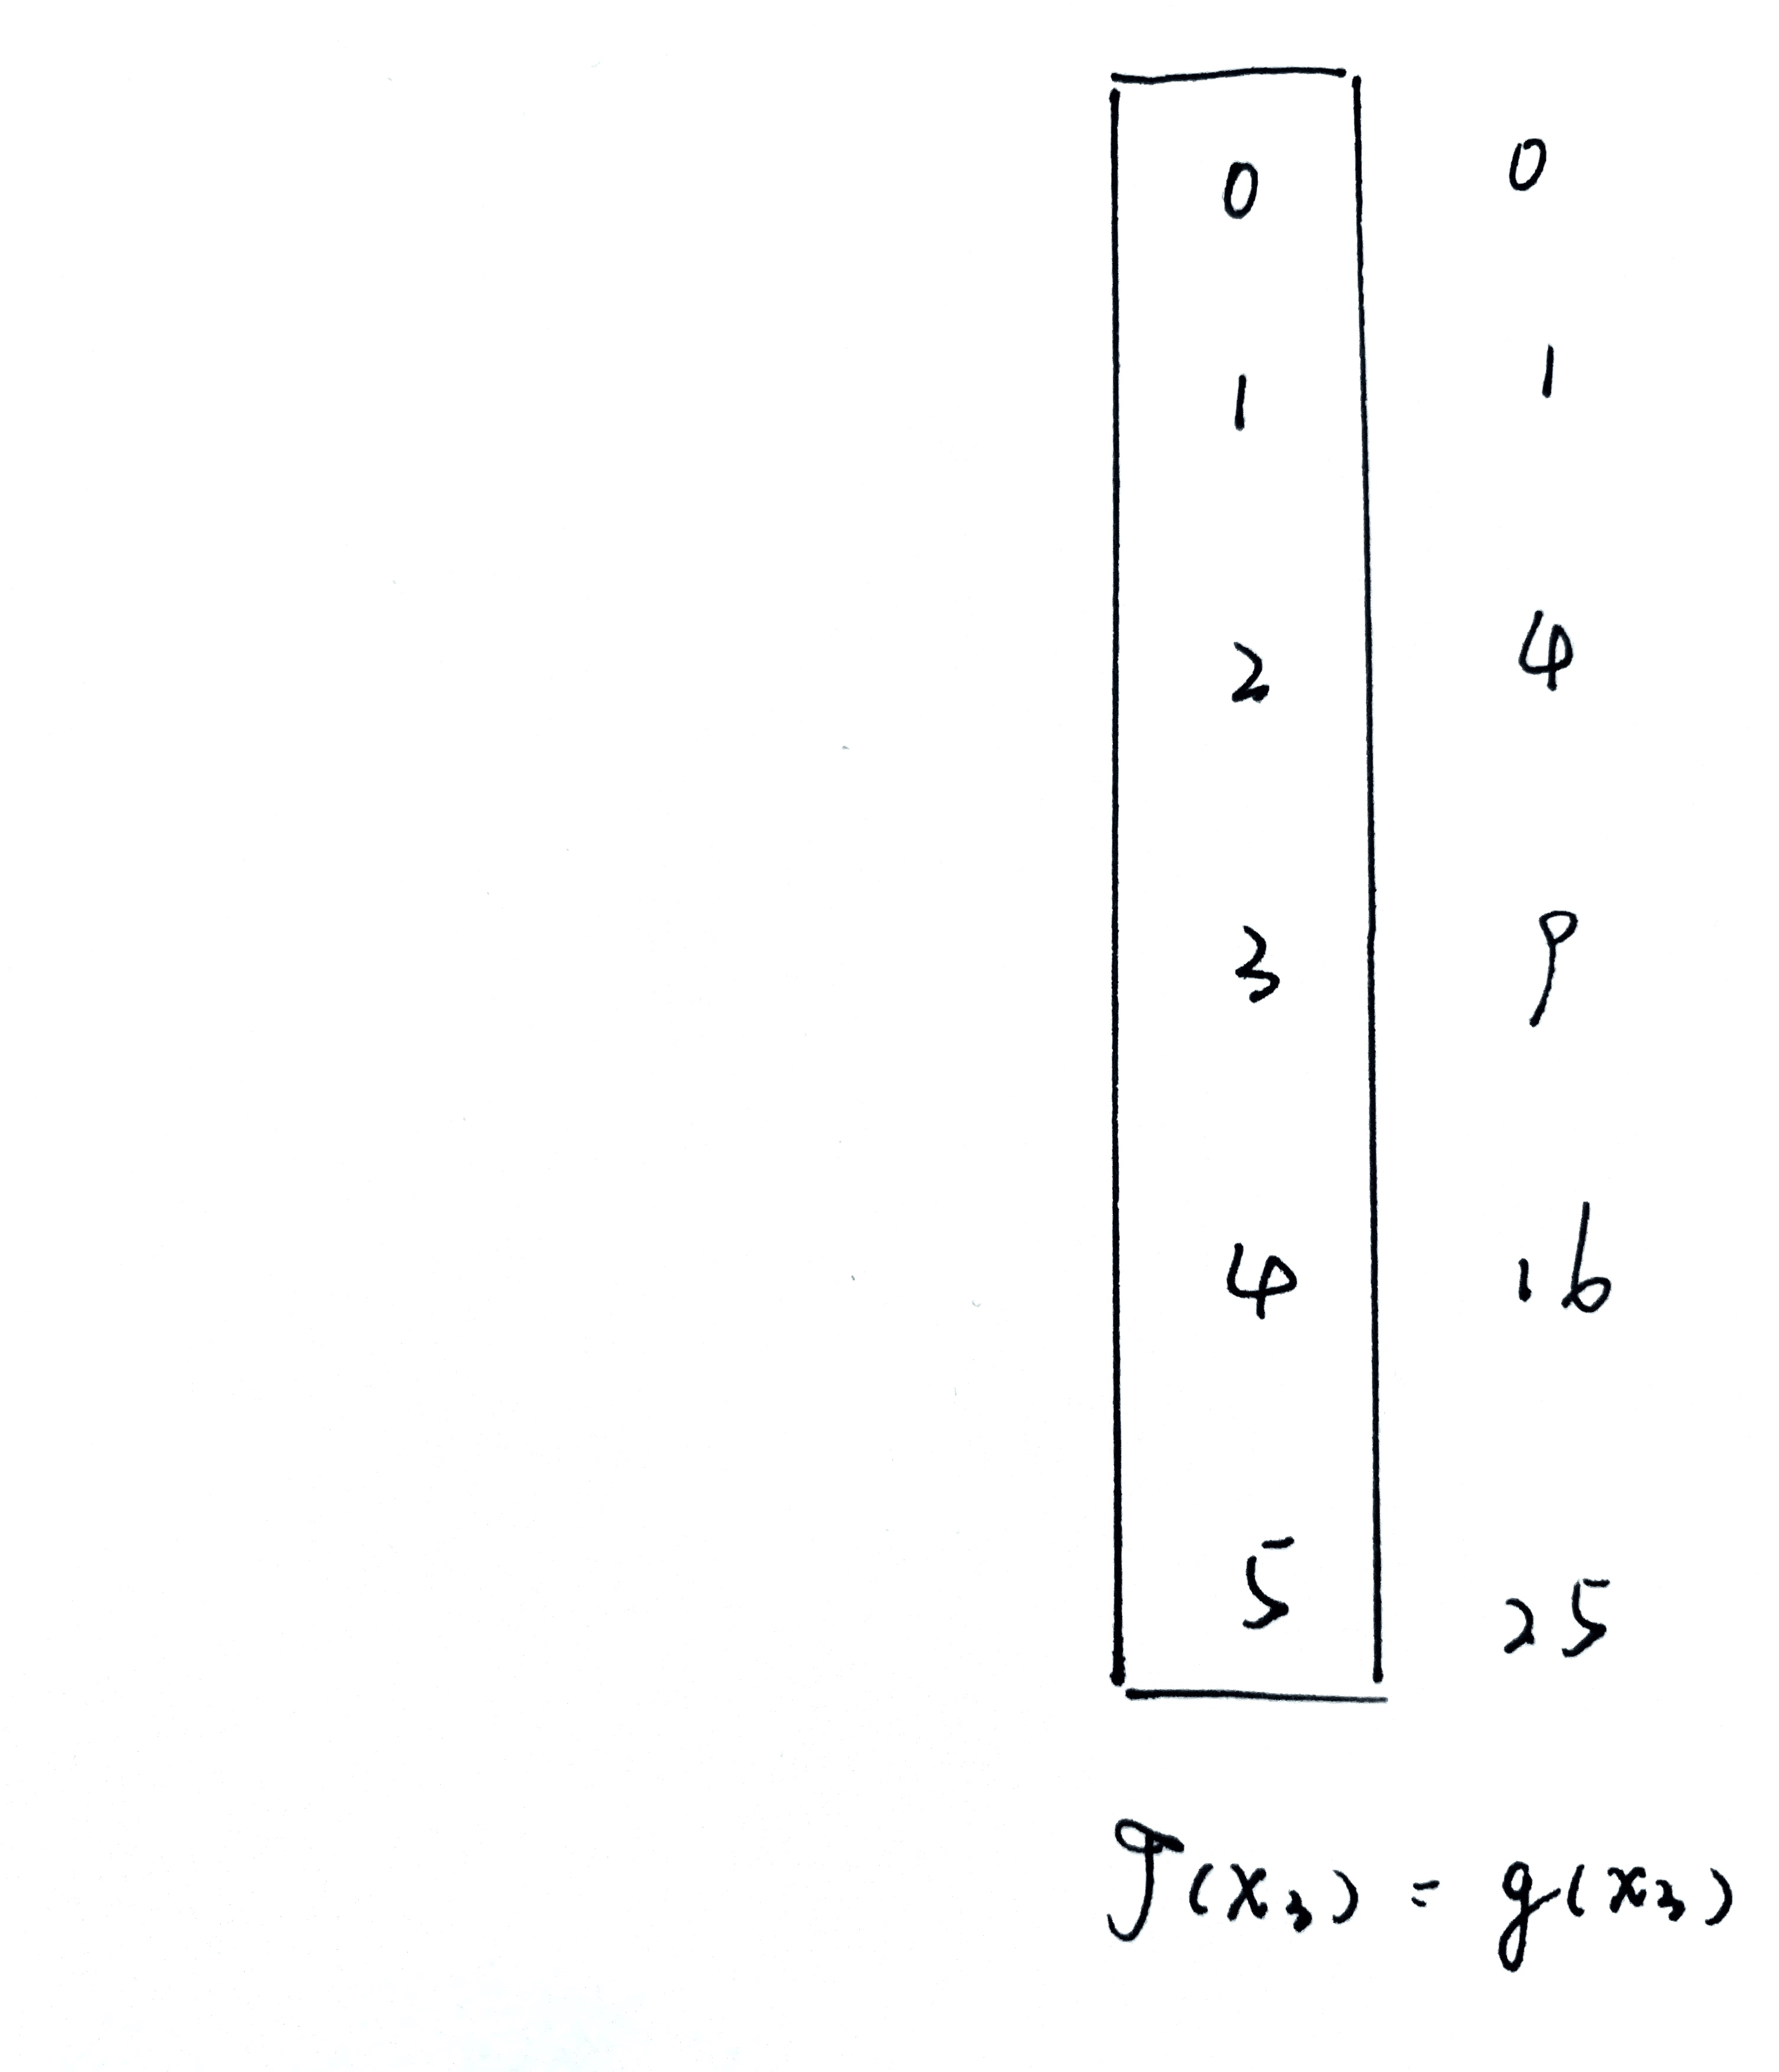
\includegraphics[width = .3\textwidth]{dp1.jpg}
      \caption{}
      \label{dp1}
    \end{figure}
    \item 2) For every possible state $x_2$ at stage 2 compute minimum cost to go as $\ref{dp2}$;
    \begin{figure}[htbp]
      \centering
      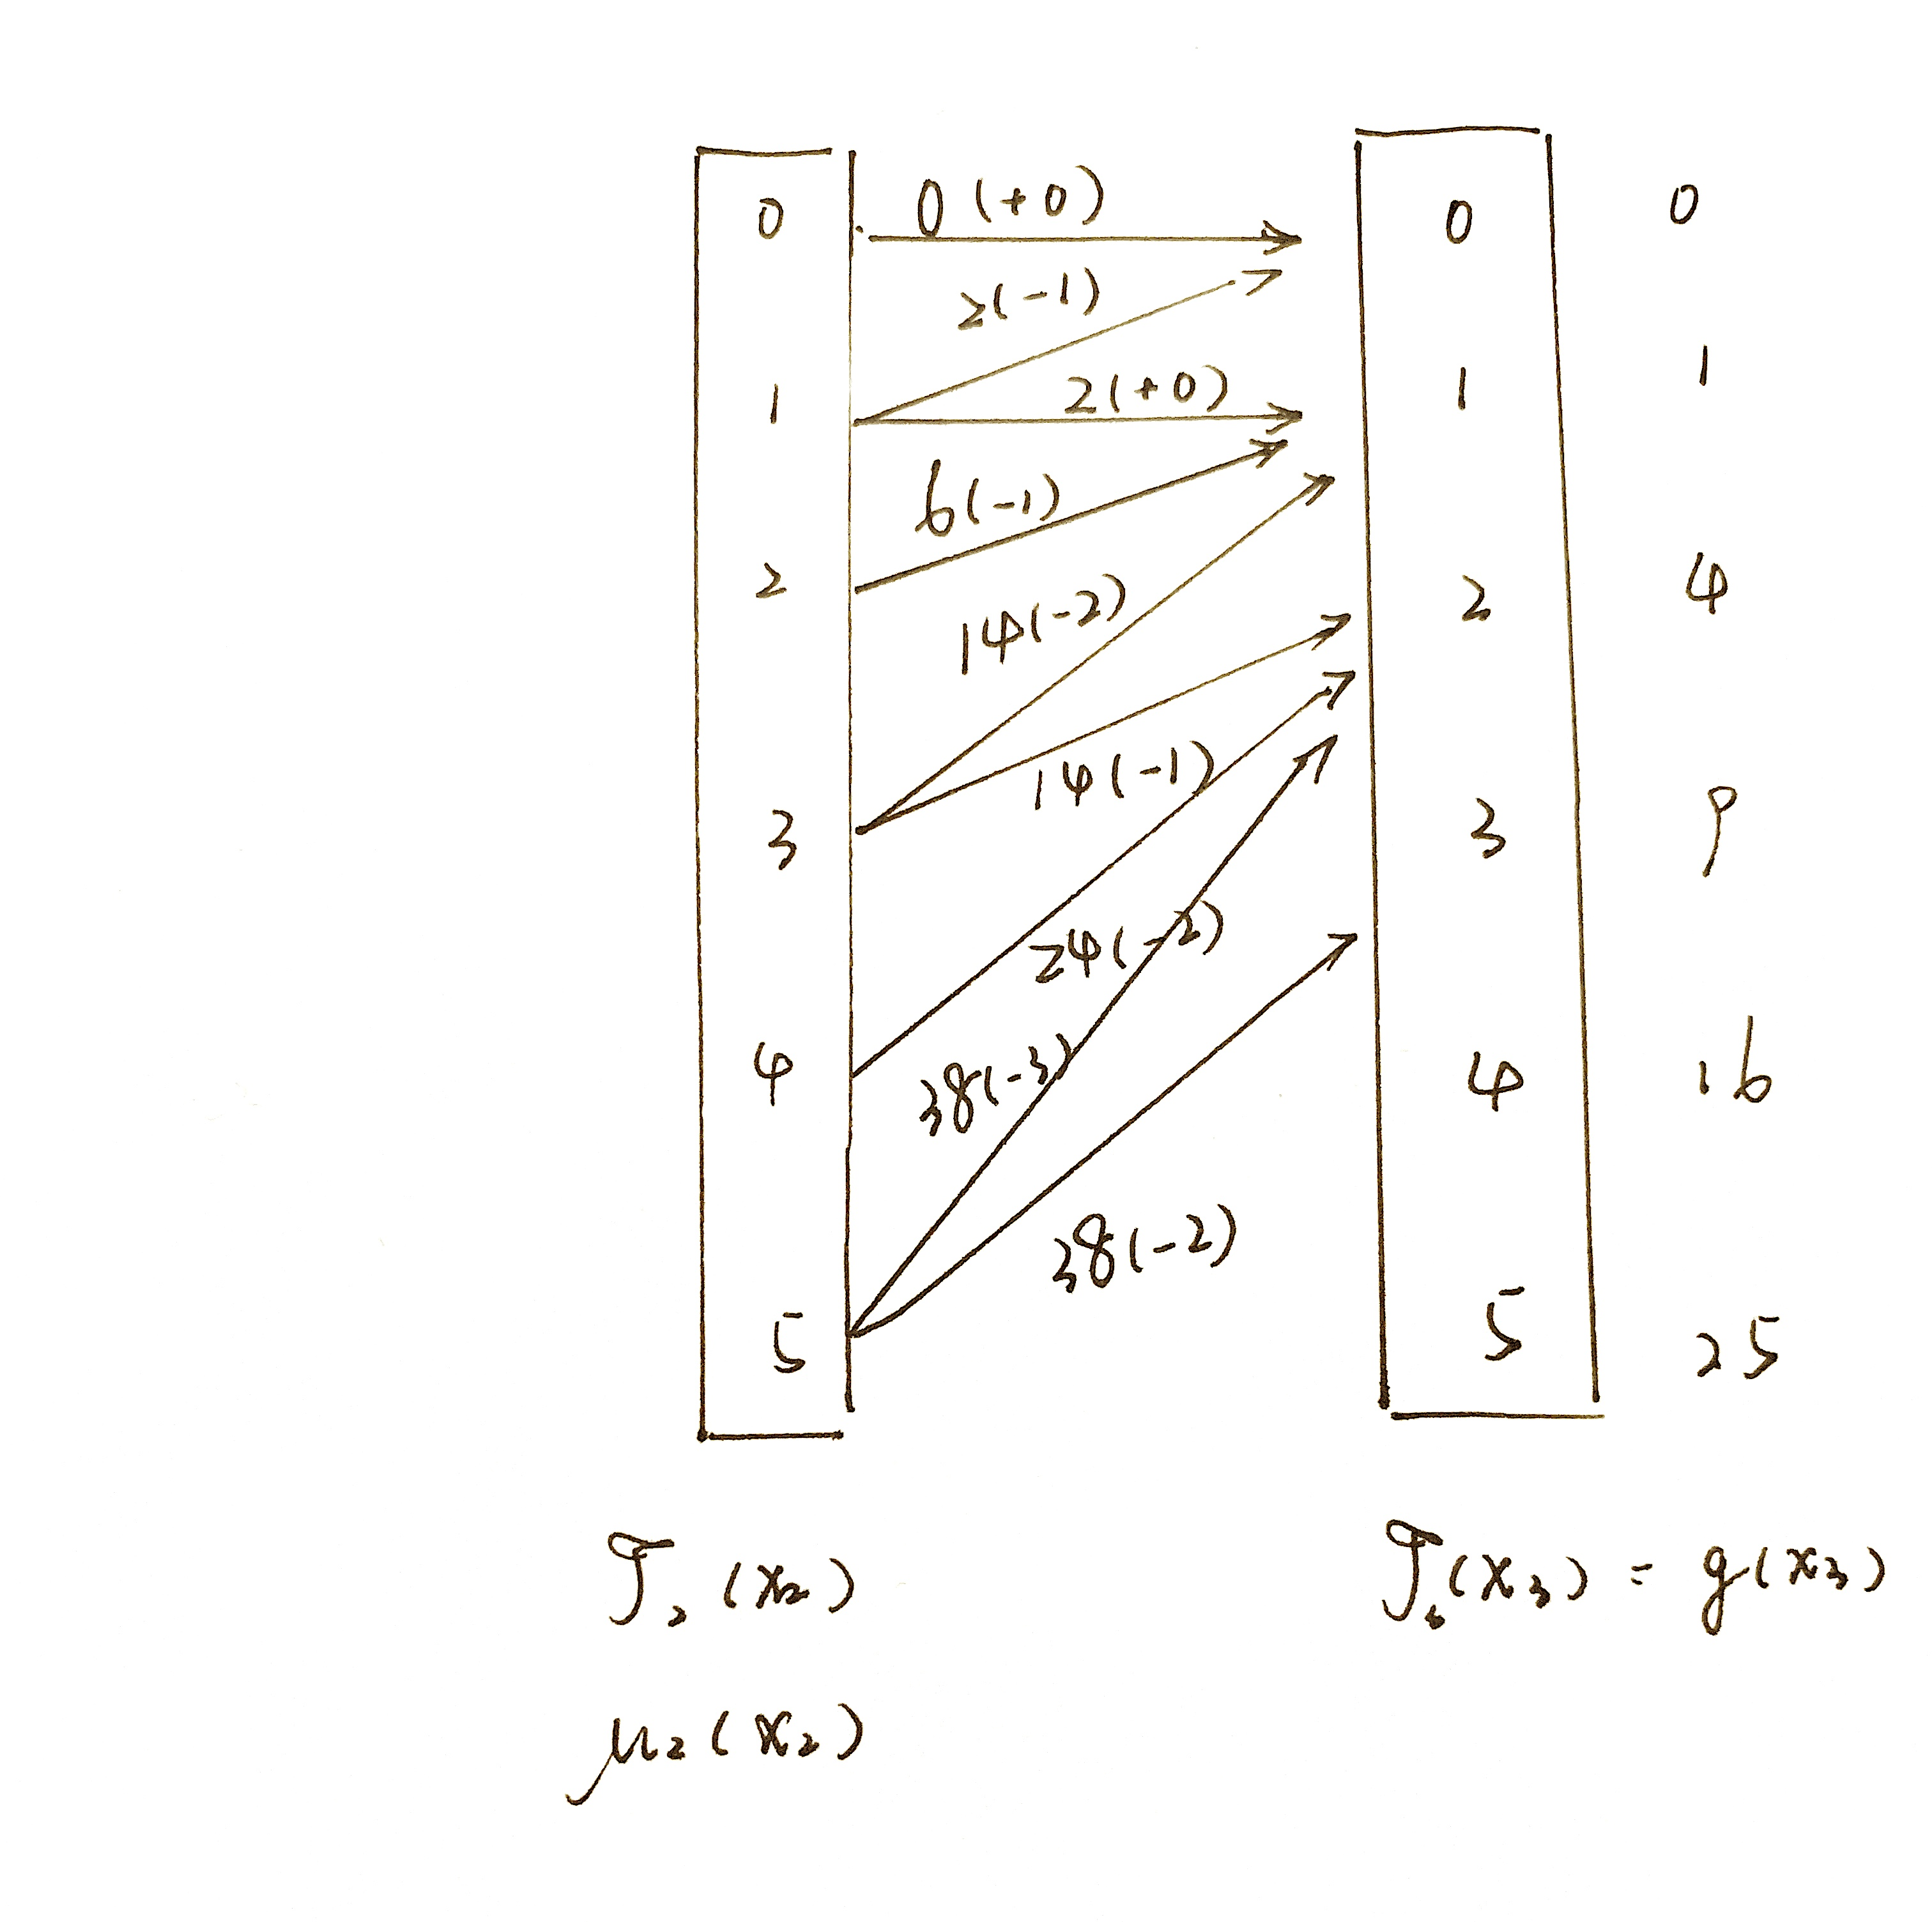
\includegraphics[width = .35\textwidth]{dp2.jpg}
      \caption{}
      \label{dp2}
    \end{figure}
    \item 3) For every possible state $x_1$ at stage 2 compute minimum cost to go as $\ref{dp3}$;
    \begin{figure}[htbp]
      \centering
      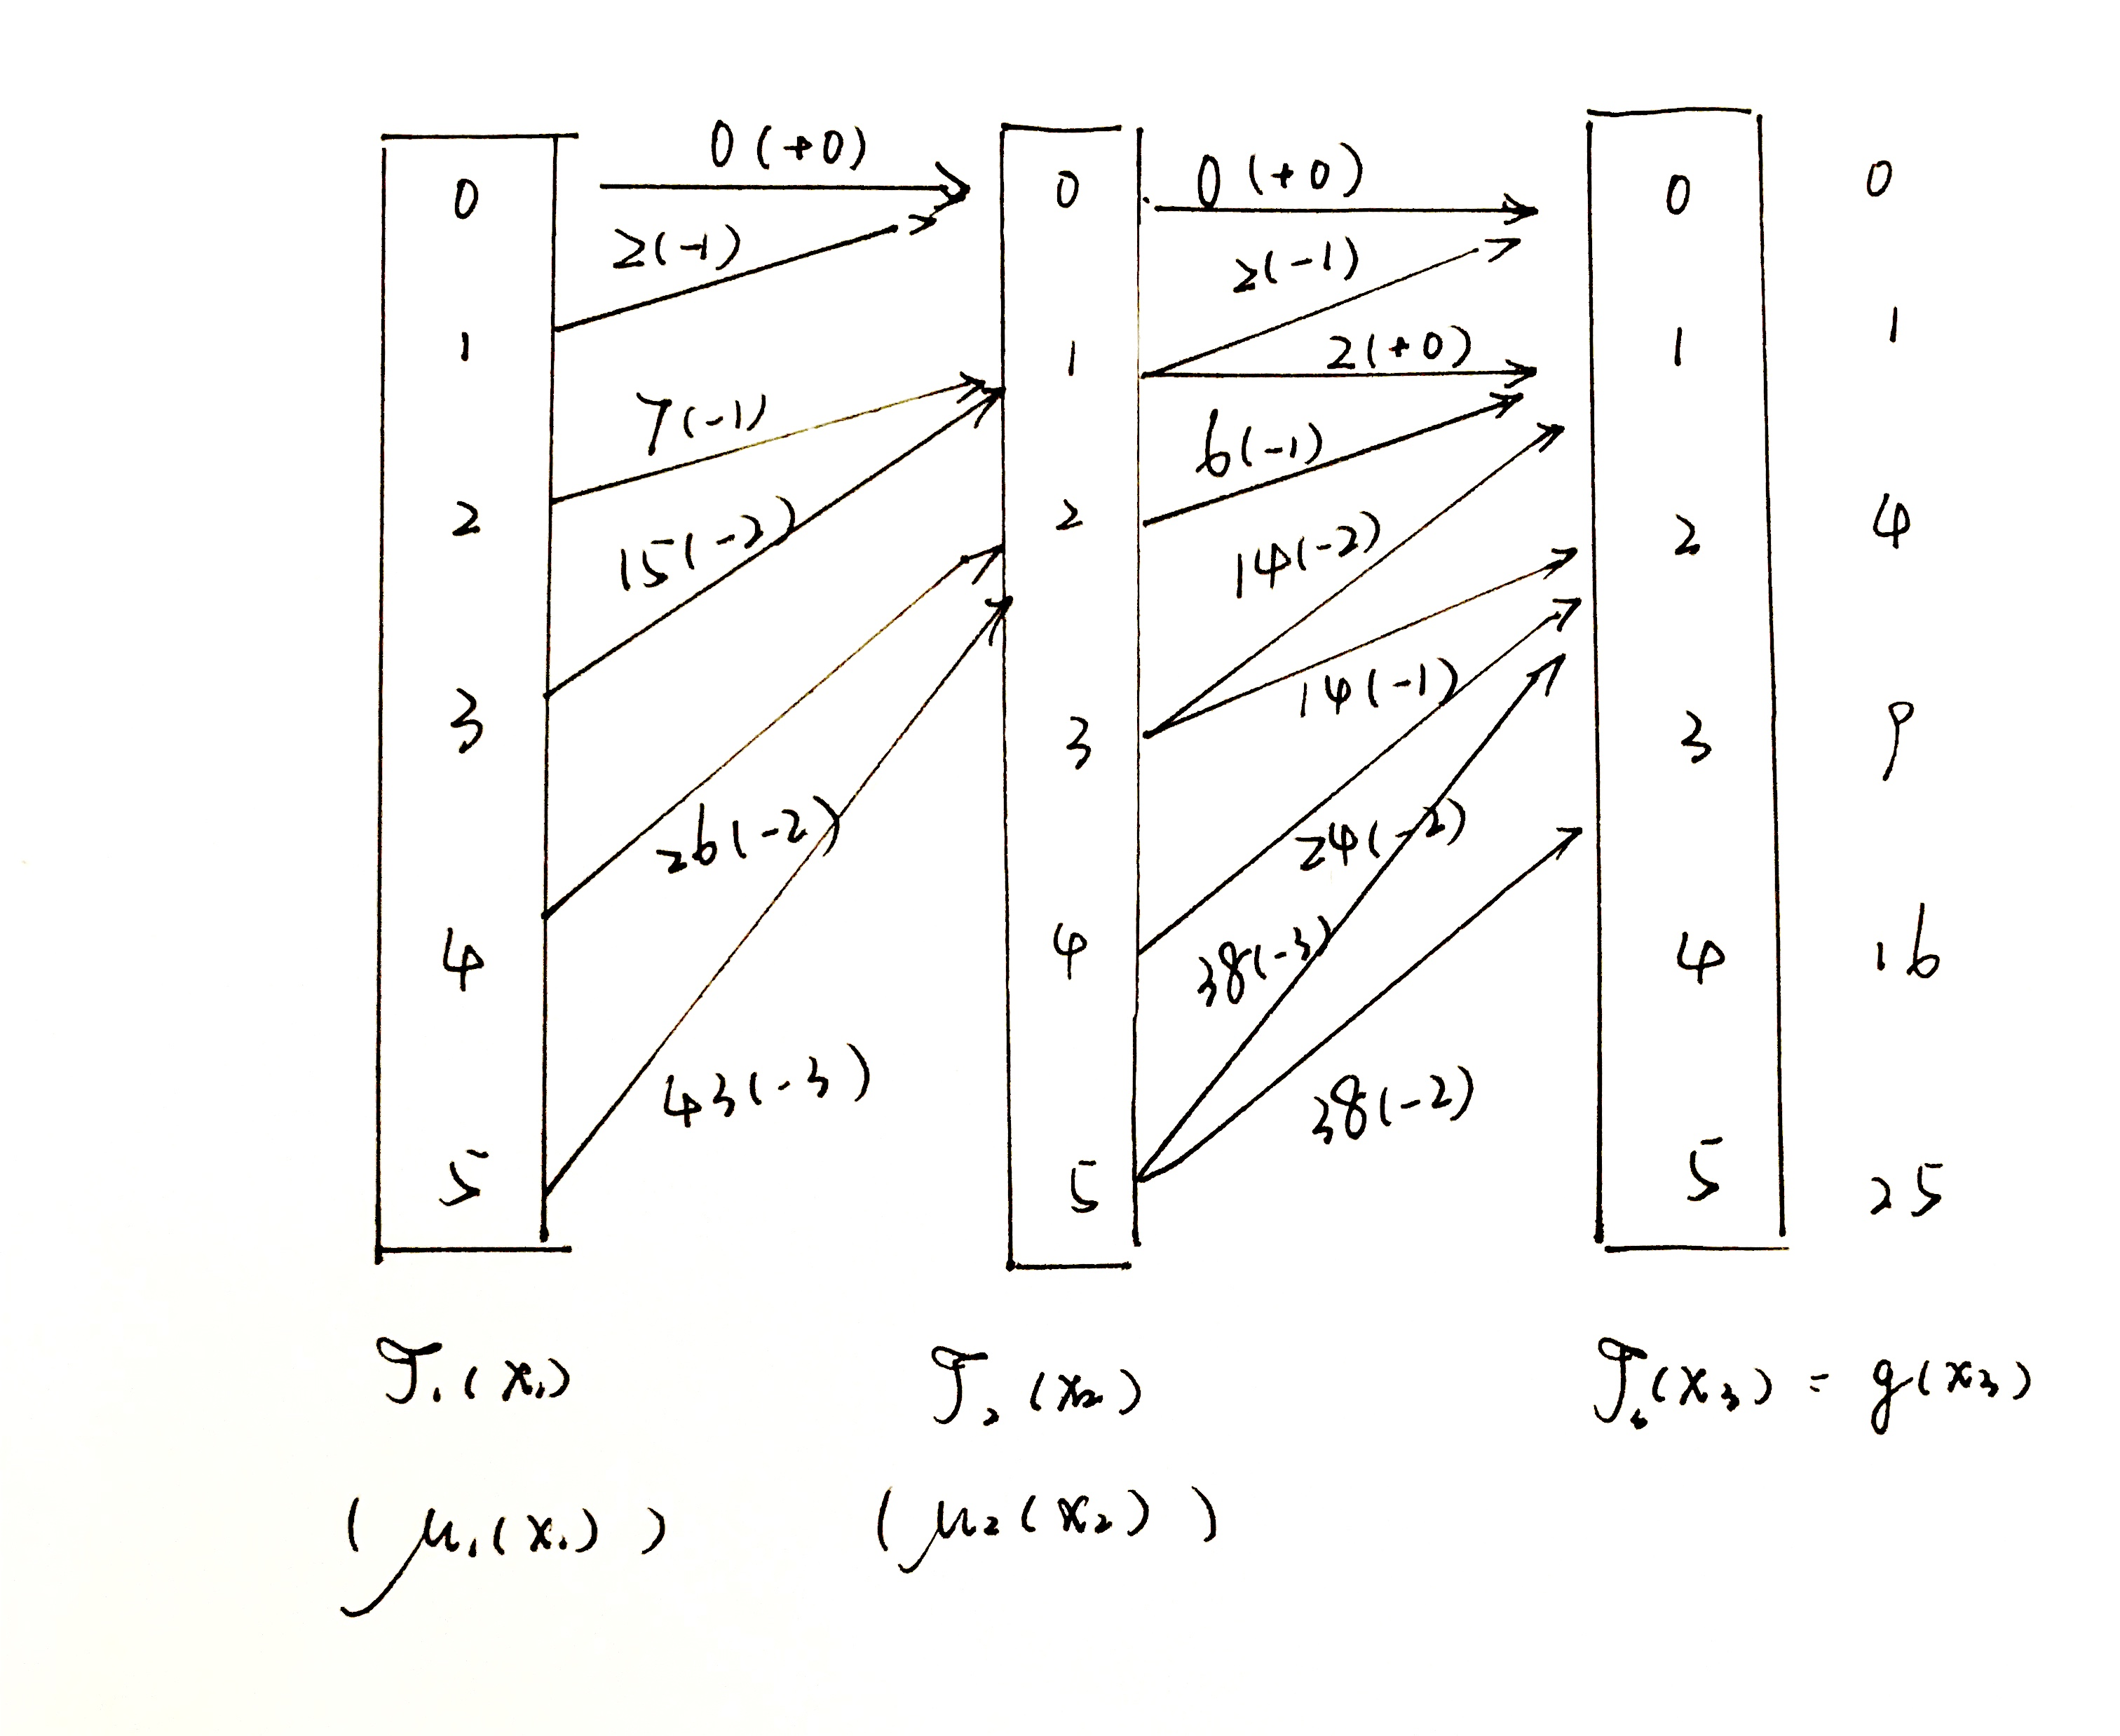
\includegraphics[width = .58\textwidth]{dp3.jpg}
      \caption{}
      \label{dp3}
    \end{figure}
    \item 4) For state $x_0$ at stage 0, compute the minimum cost to go as $\ref{dp4}$
    \begin{figure}[htbp]
      \centering
      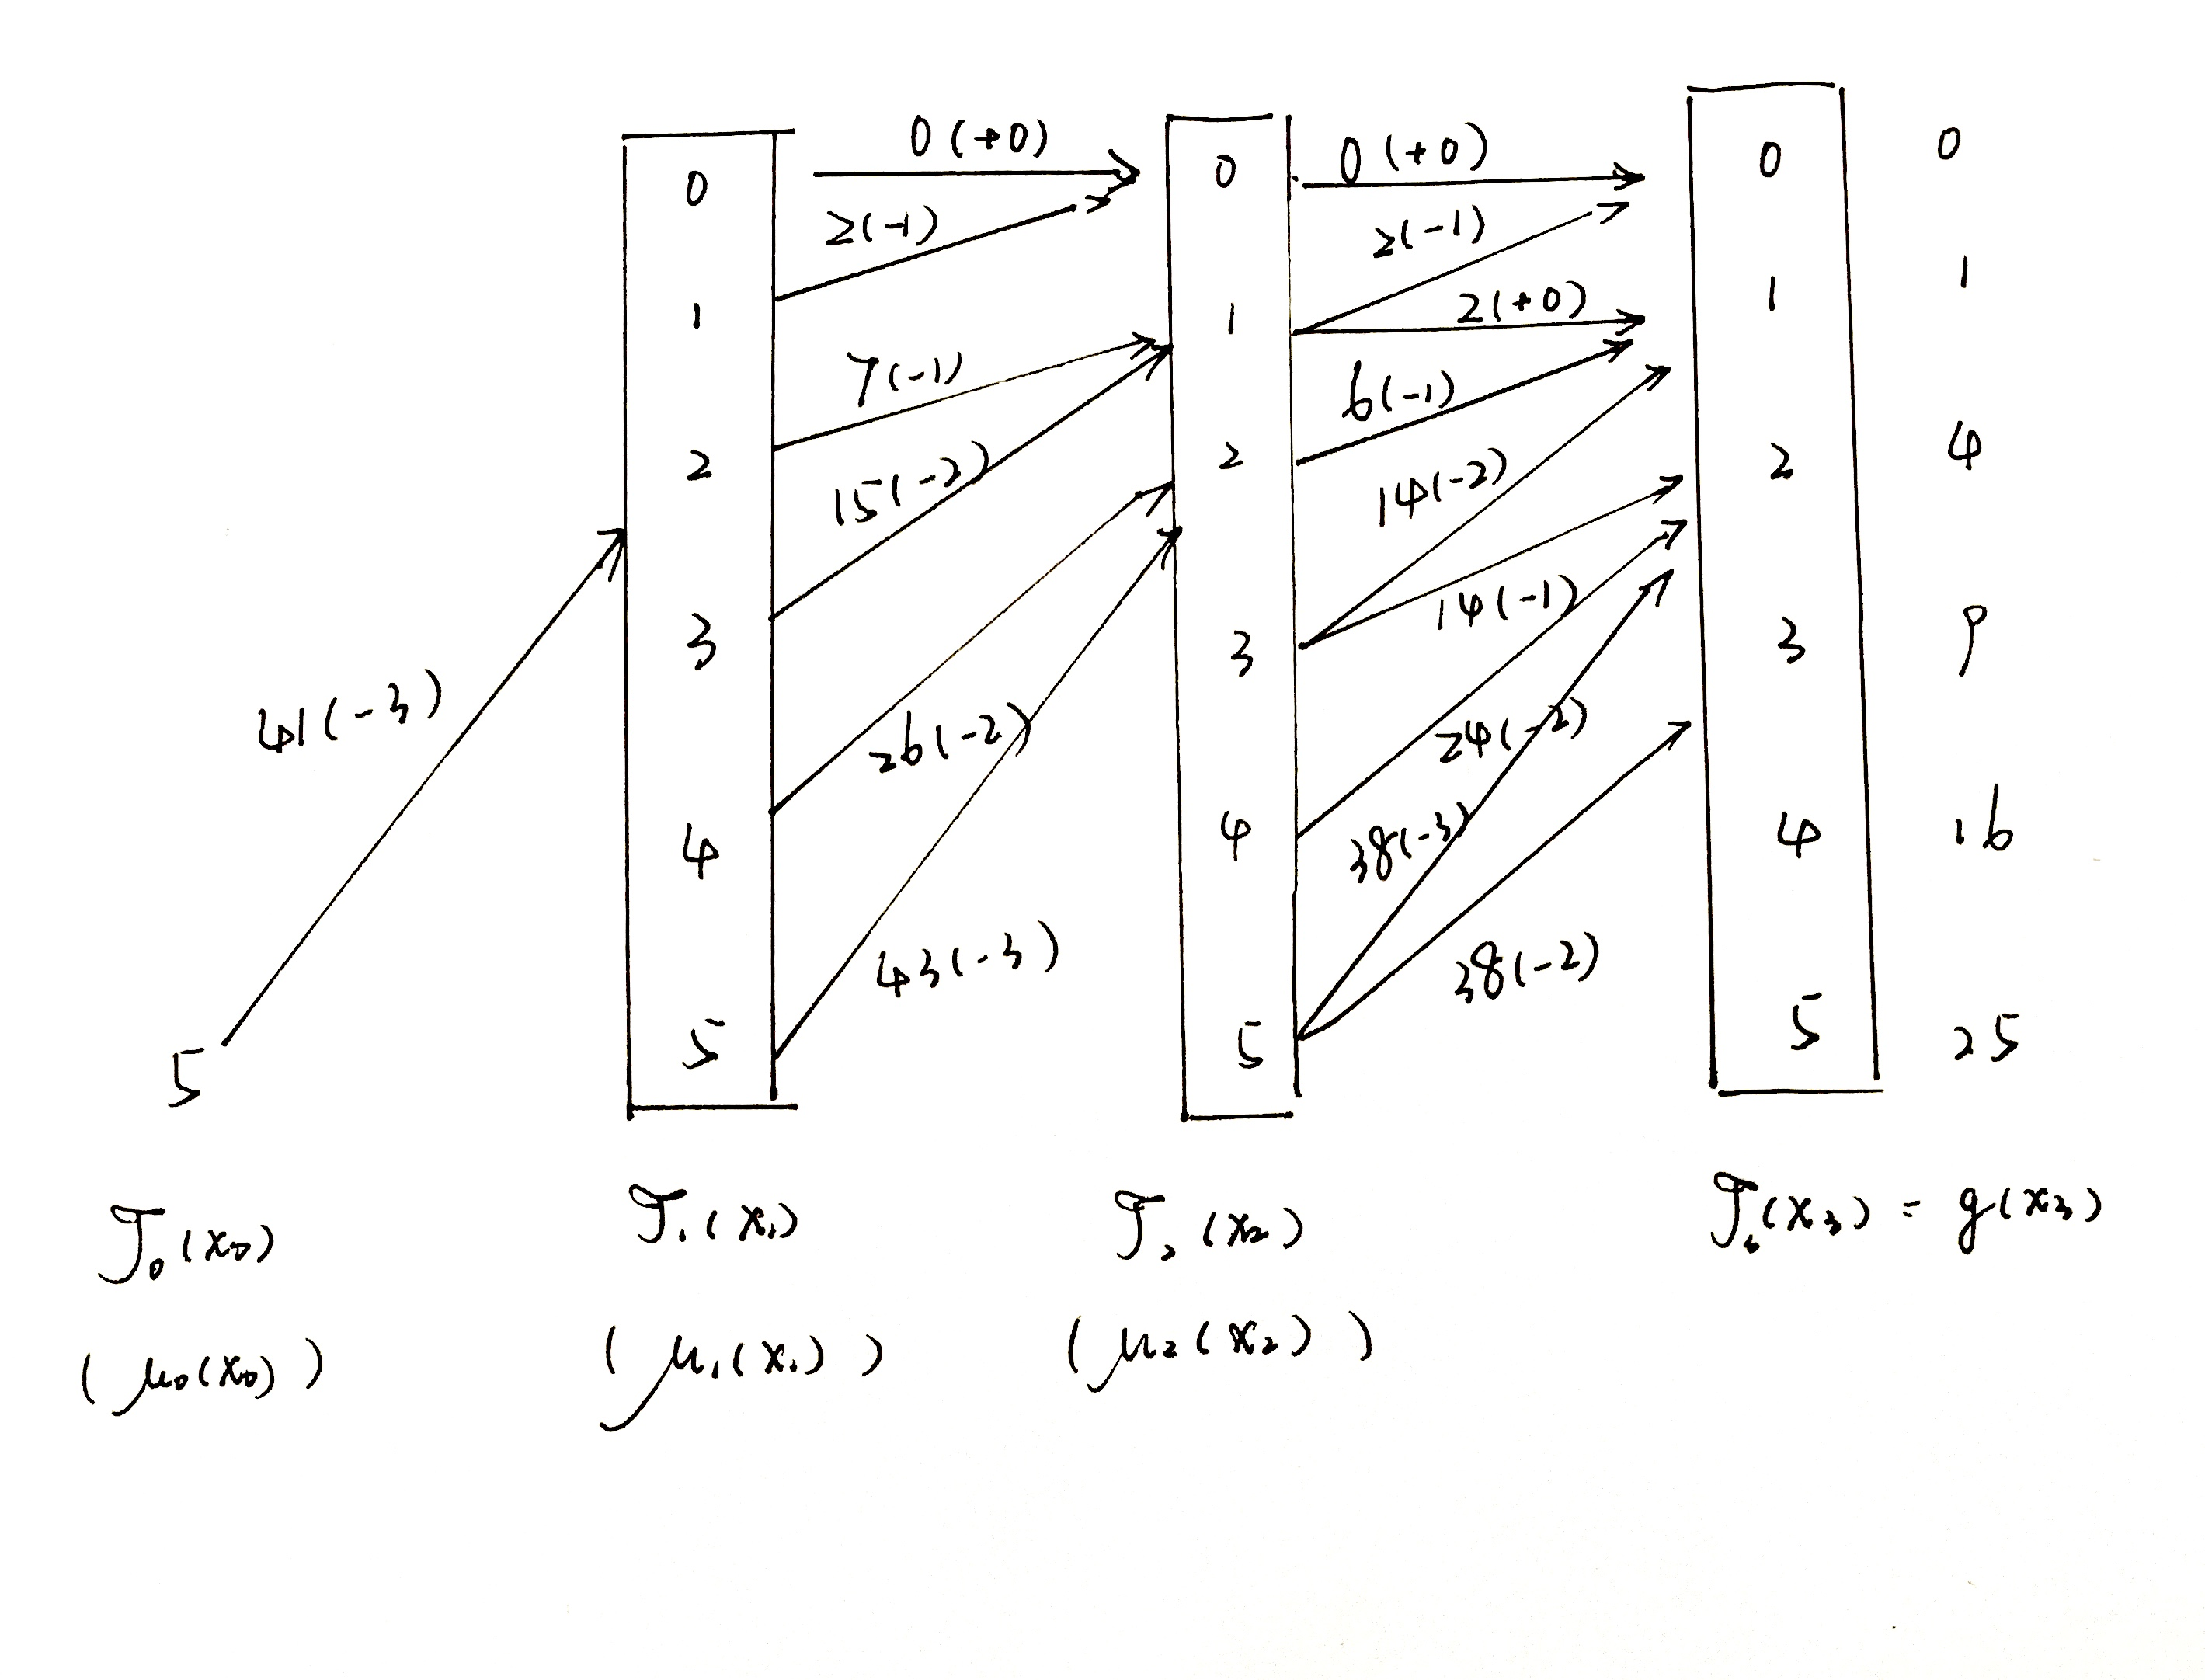
\includegraphics[width = .58\textwidth]{dp4.jpg}
      \caption{}
      \label{dp4}
    \end{figure} 
  \end{itemize}
  
  Correction: (* Sorry I was making a mistake, the cost from $x_1 = 5$ to $x_2 = 2$ is 40, though it does not affect the final results)

   
Instead of doing DP we can formulate it as a finite horizon discrete-time Riccatti equation, 
\begin{equation}
  \begin{aligned}
  \min \ &x^{\top}_NQ_Nx_N + \sum_{k=0}^{N = 3} x^{\top}_kQ_kx_k + u^{\top}_kR_ku_k  \\
  s.t. \ &x_n = A_n x_n + B_n u_n 
  \end{aligned}
\end{equation}
where $Q_n = R_n = A_n = B_n= 1 \  \forall n \in \{0,1,2,3\},$ so apply the solution to 
Riccatti equation as follows:
\begin{equation}
  \begin{aligned}
  &P_N = Q_N  = 1 \\ \nonumber
  &K_n = -(B_n^{\top} P_{n+1}B_n + R_n)^{-1}B_n^{\top} P_{n+1}A_n \\ \nonumber
  &Pn = Q_n + A^{\top}_n P_{n+1}A_n + A_n^{\top} P_{n+1}B_nK_n \\ \nonumber
  &u^{*}_n = K_n x_n \\ \nonumber
  &J^{*} = x_0^{\top} P_0 x_0    \\ \nonumber
  \end{aligned}
\end{equation}
we get: $P_3 = 1$, $K_2 = \frac{1}{2}$, $P_2 = \frac{3}{2}$, $K_1 = -\frac{3}{5}$, $P_1 = \frac{8}{5}$,
$K_1 = -\frac{8}{13}$, with a little approximation the state sequence should be ${x_0 = 5, x_1 = 2, x_2 = 1, x_3 = 0}$ or ${x_0 = 5, x_1 = 2, x_2 = 1, x_3 = 1}$,
while the policy squence shouldbe ${u_0 = -3, u_1 = -1, u_2 = -1}$ or ${u_0 = -3, u_1 = -1, u_2 = 0}$, the optimal cost value $J^{*} = 41$. 

\item[b)] While $x_3=5$ has been a constraint, the cost of the final state is fixed as 25, processing the same steps in a)
we get the optimal cost $J^{*} = 76$, the optimal sequences are  $\{x_0 = 5, u_0 = -3, x_1 = 3, u_1 = 0,$ $ x_2 = 1, u_2 = 3, x_3 = 5\}$ or 
$\{x_0 = 5, u_0 = -2, x_1 = 3, u_1 = 0, x_2 = 3, u_2 = 2, x_3 = 5\}$
\begin{figure}[htbp]
  \centering
  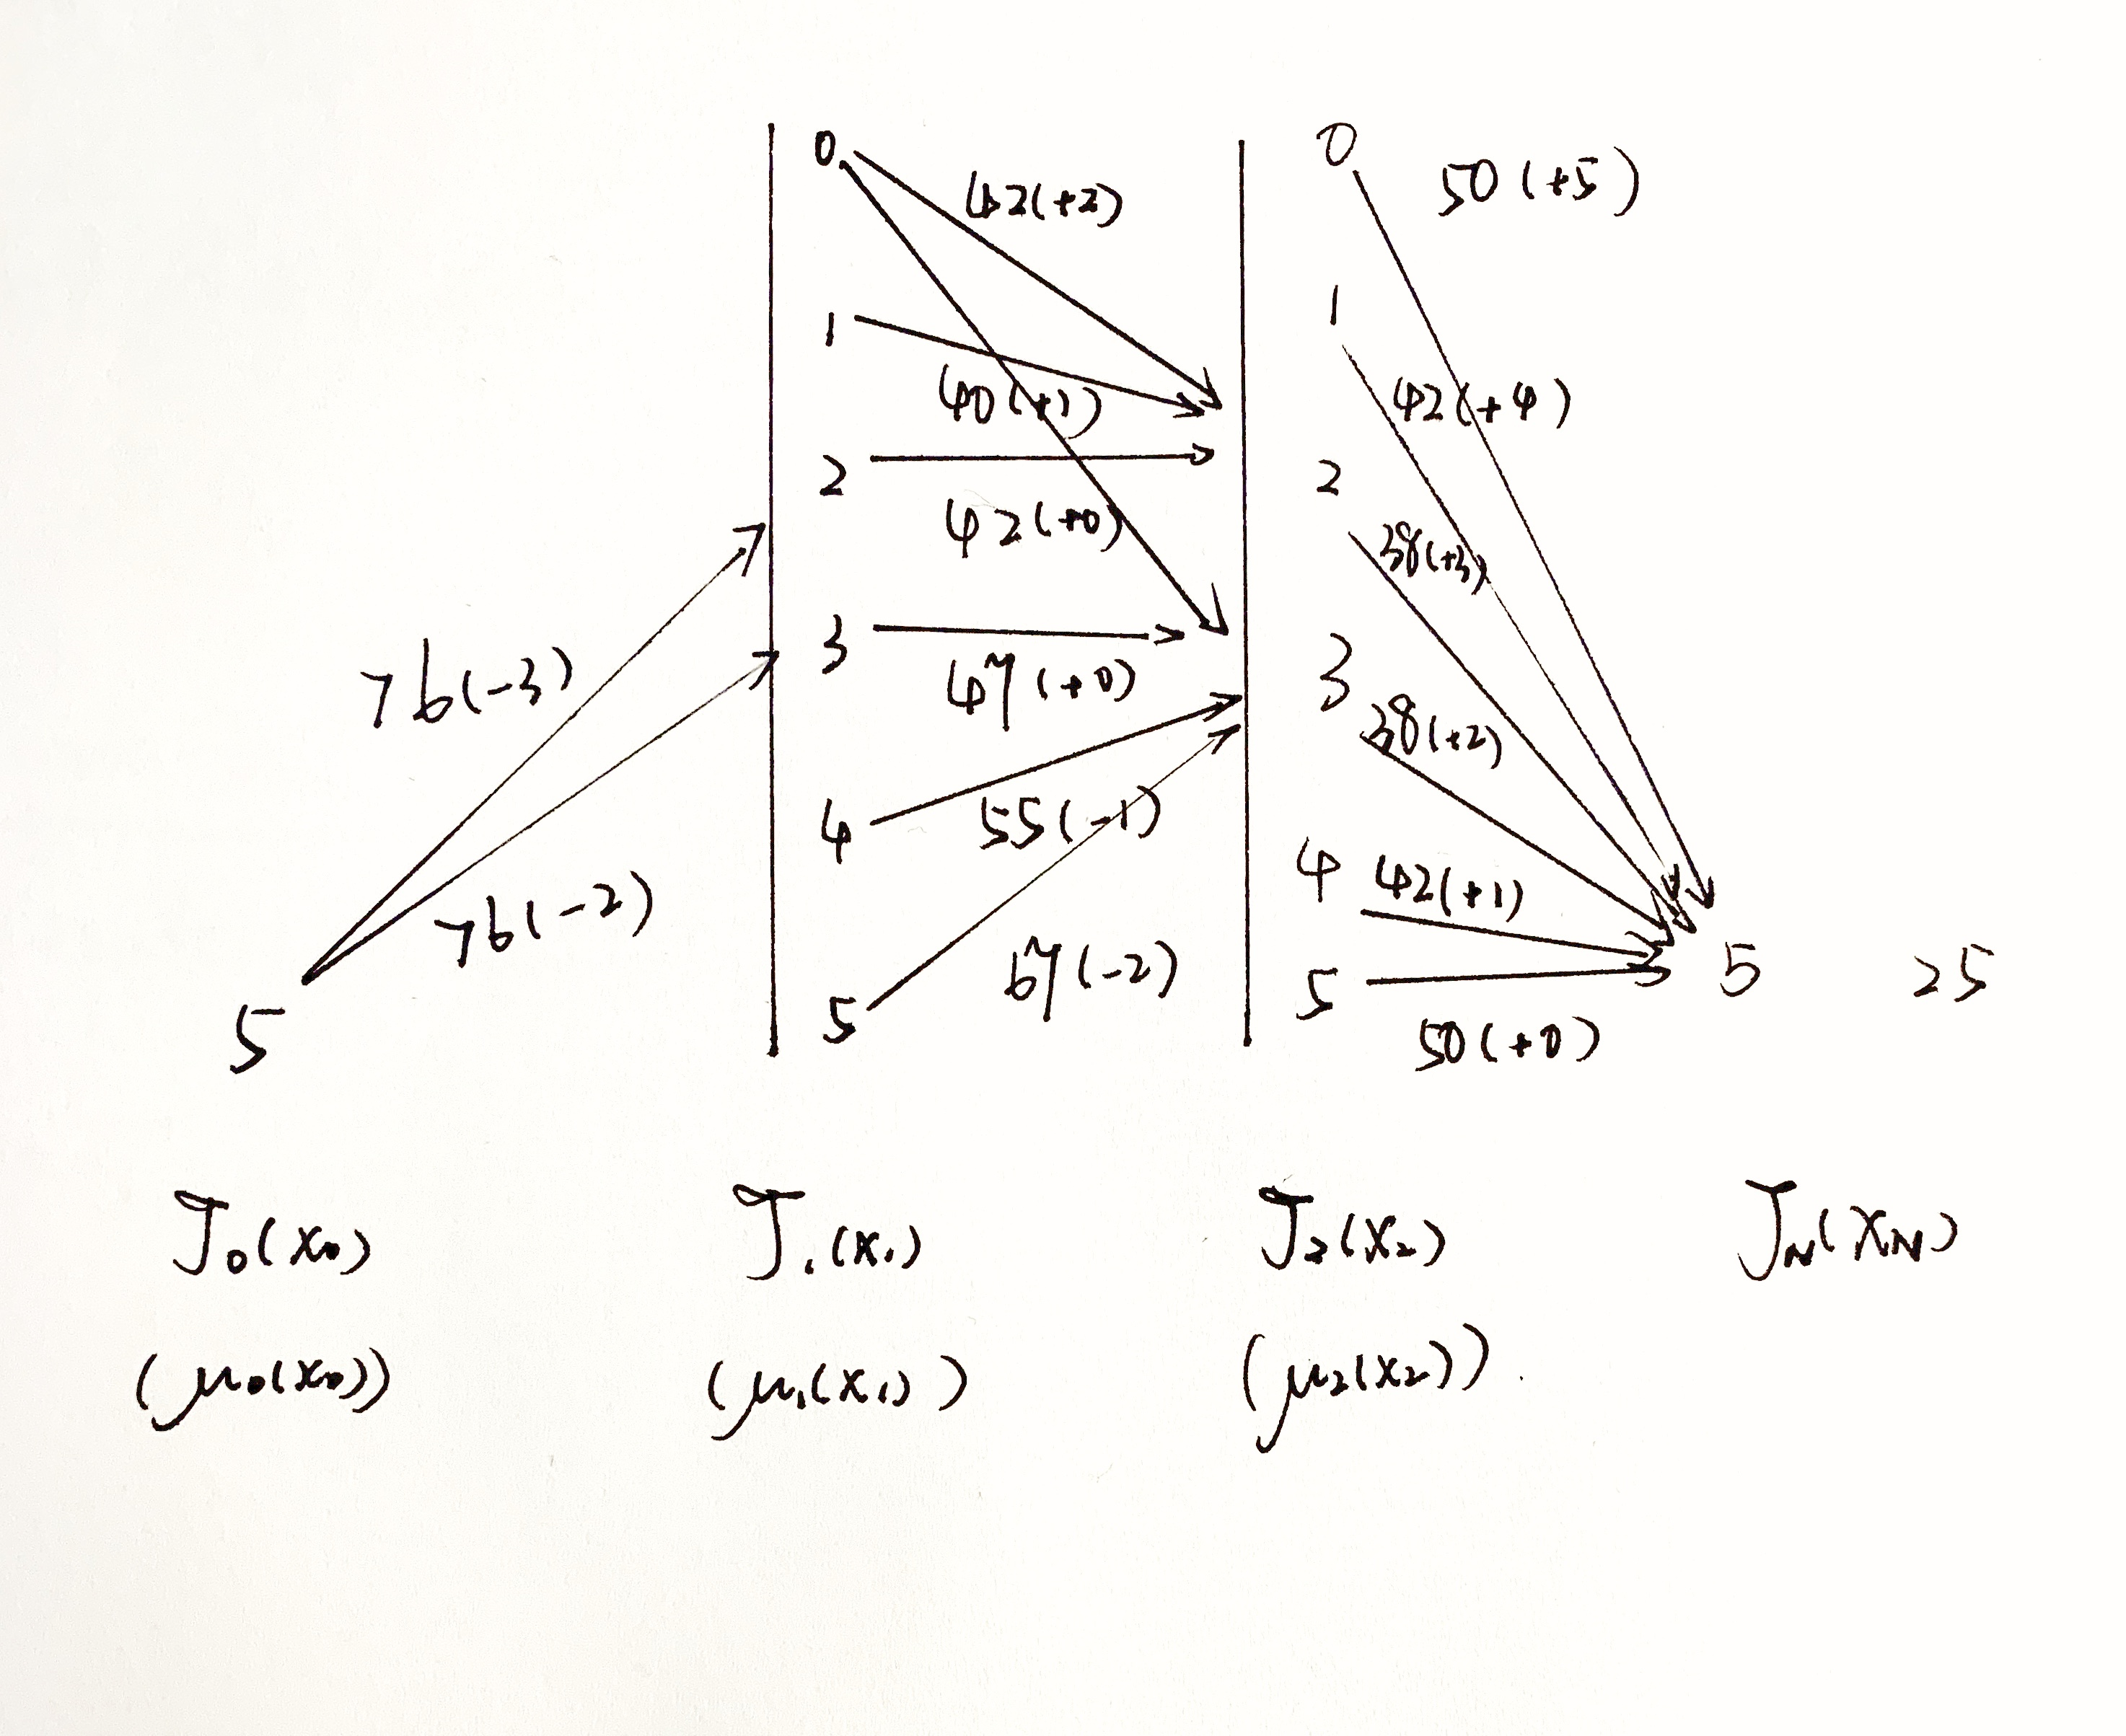
\includegraphics[width = .58\textwidth]{dp5.jpg}
  \caption{}
  \label{dp5}
\end{figure} 
\item[c)] if there's a stochastic term $w_n$, the DP process will be minimizing the expectation at each time step, as $\ref{dp6}$ shows.
\begin{figure}[htbp]
  \centering
  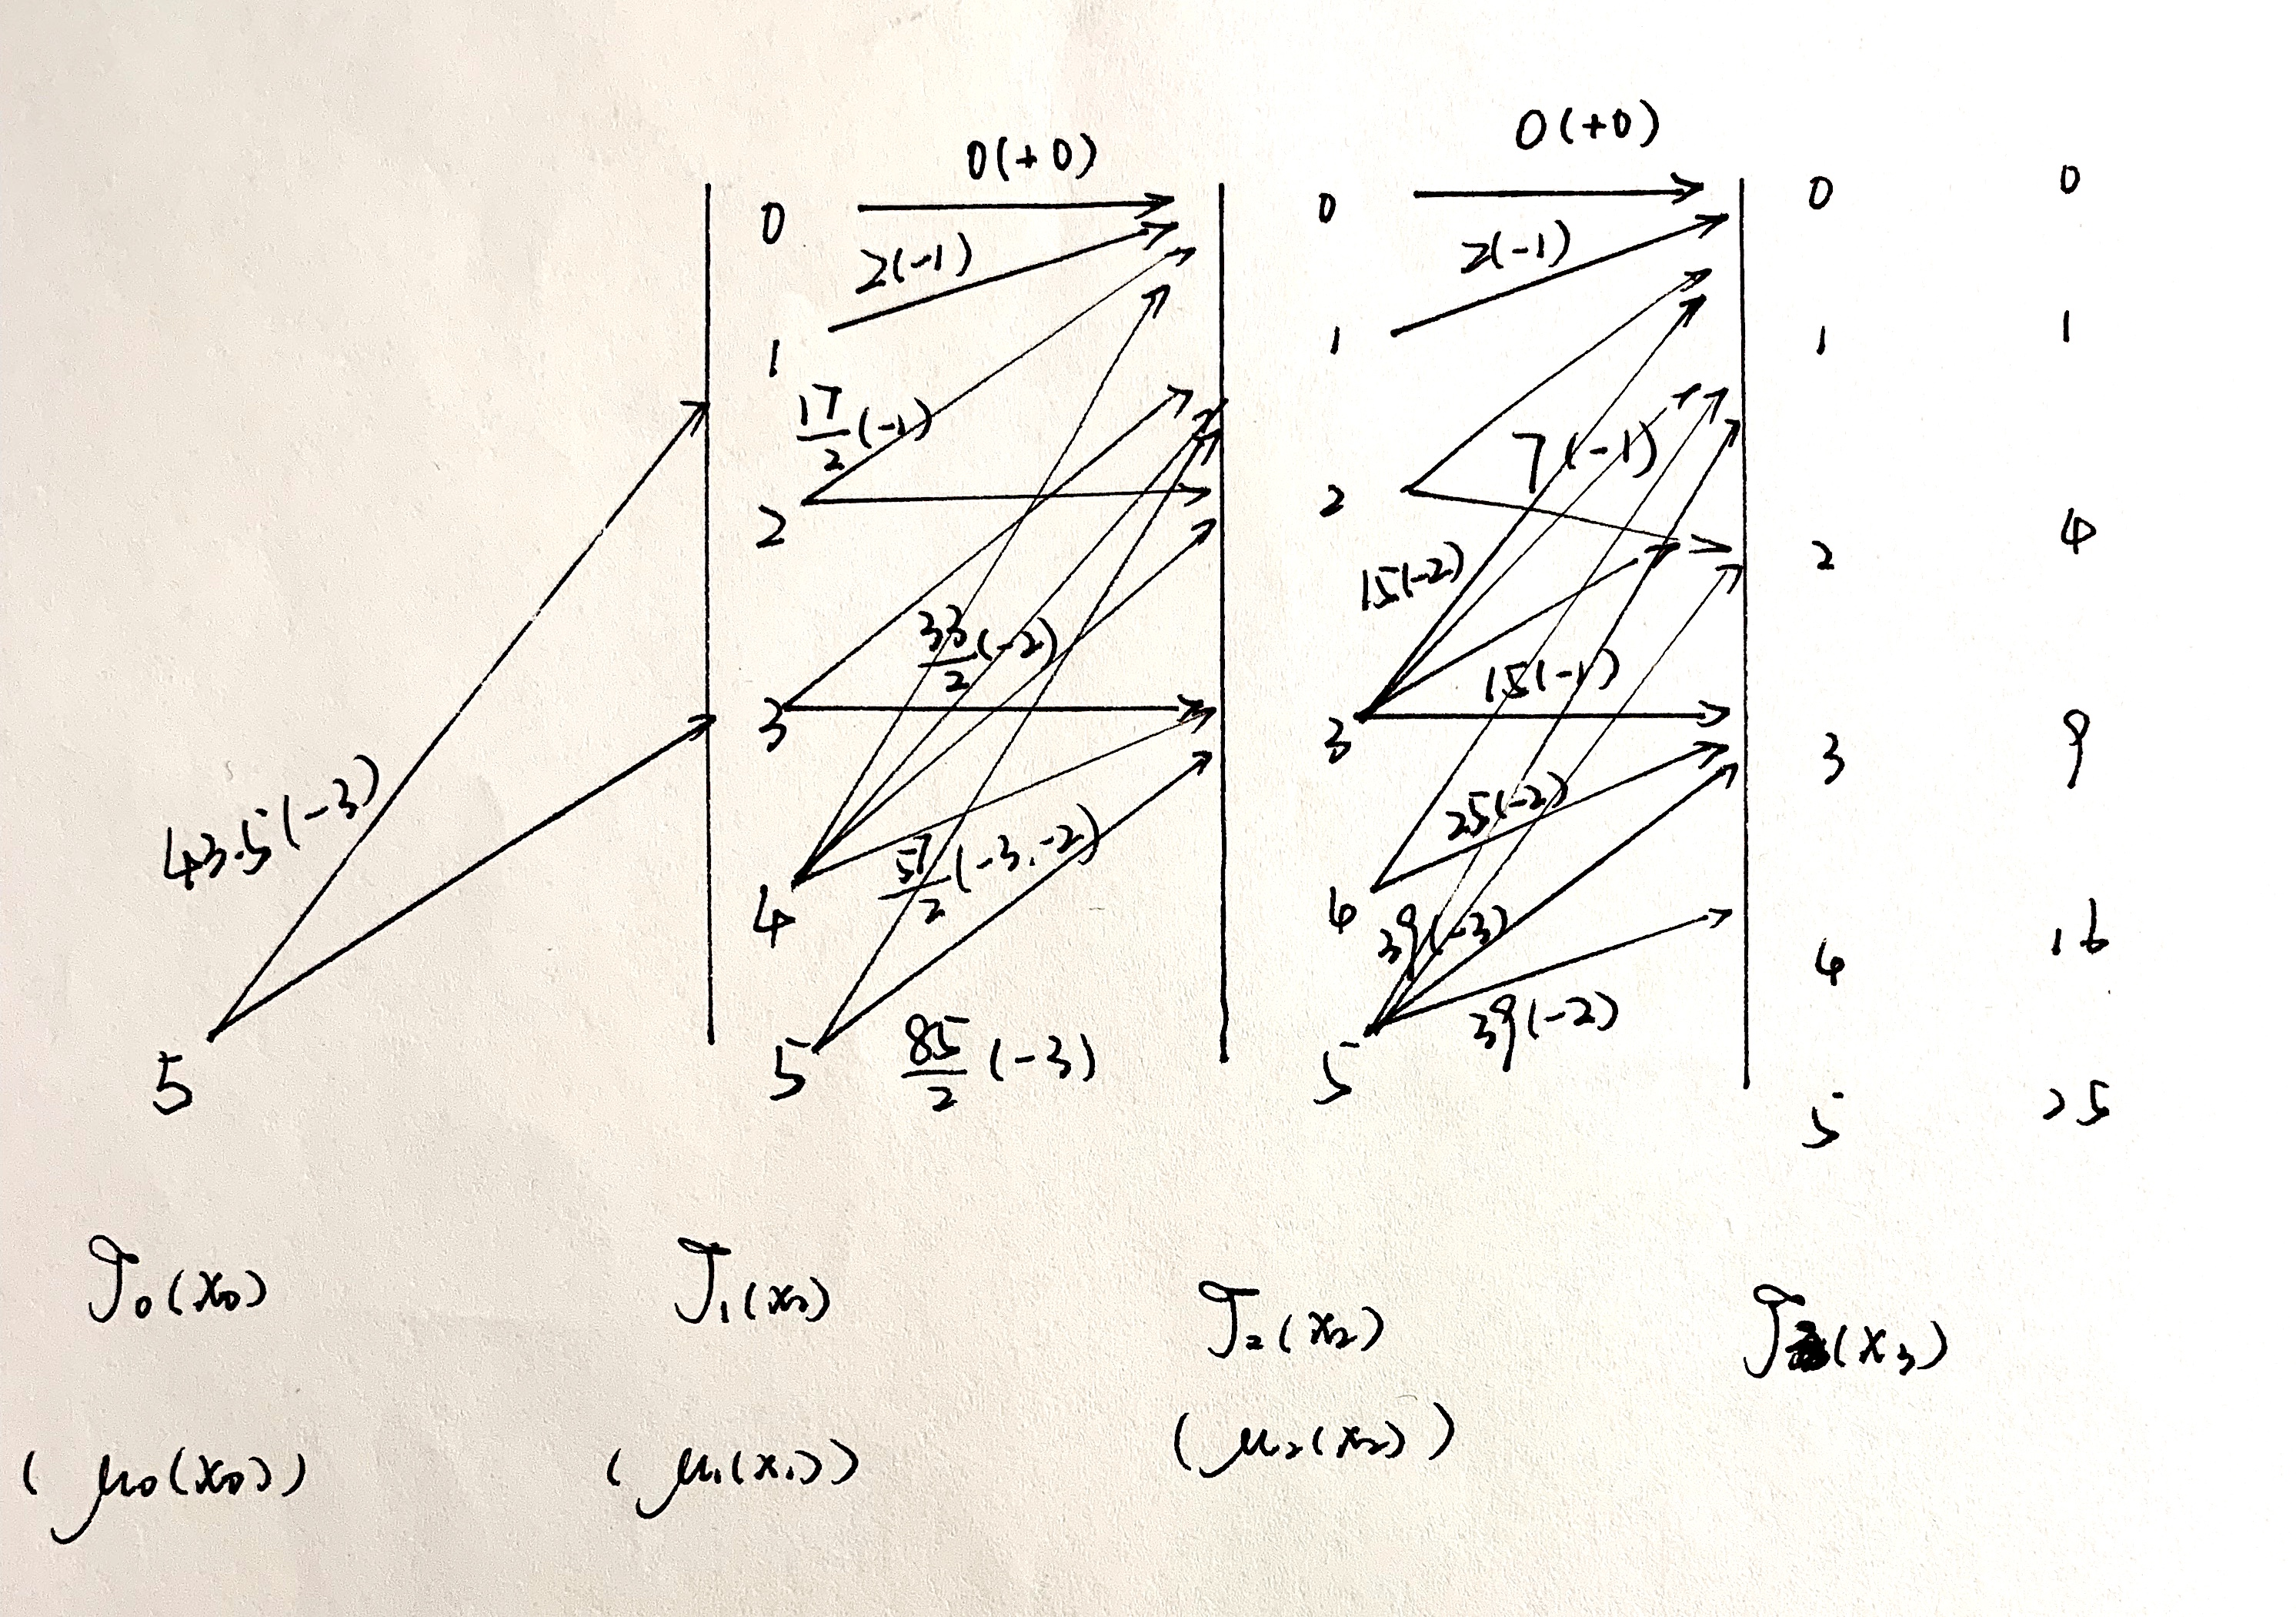
\includegraphics[width = .8\textwidth]{dp6.jpg}
  \caption{}
  \label{dp6}
\end{figure}  
$\ref{dp7}$ shows the possible paths, note that the cost of each path is not equal, the optimal one is ${x_0 = 5, x_1 = 1, x_2 = 0, x_3 = 0}$, which we cannot ensure.
\begin{figure}[htbp]
  \centering
  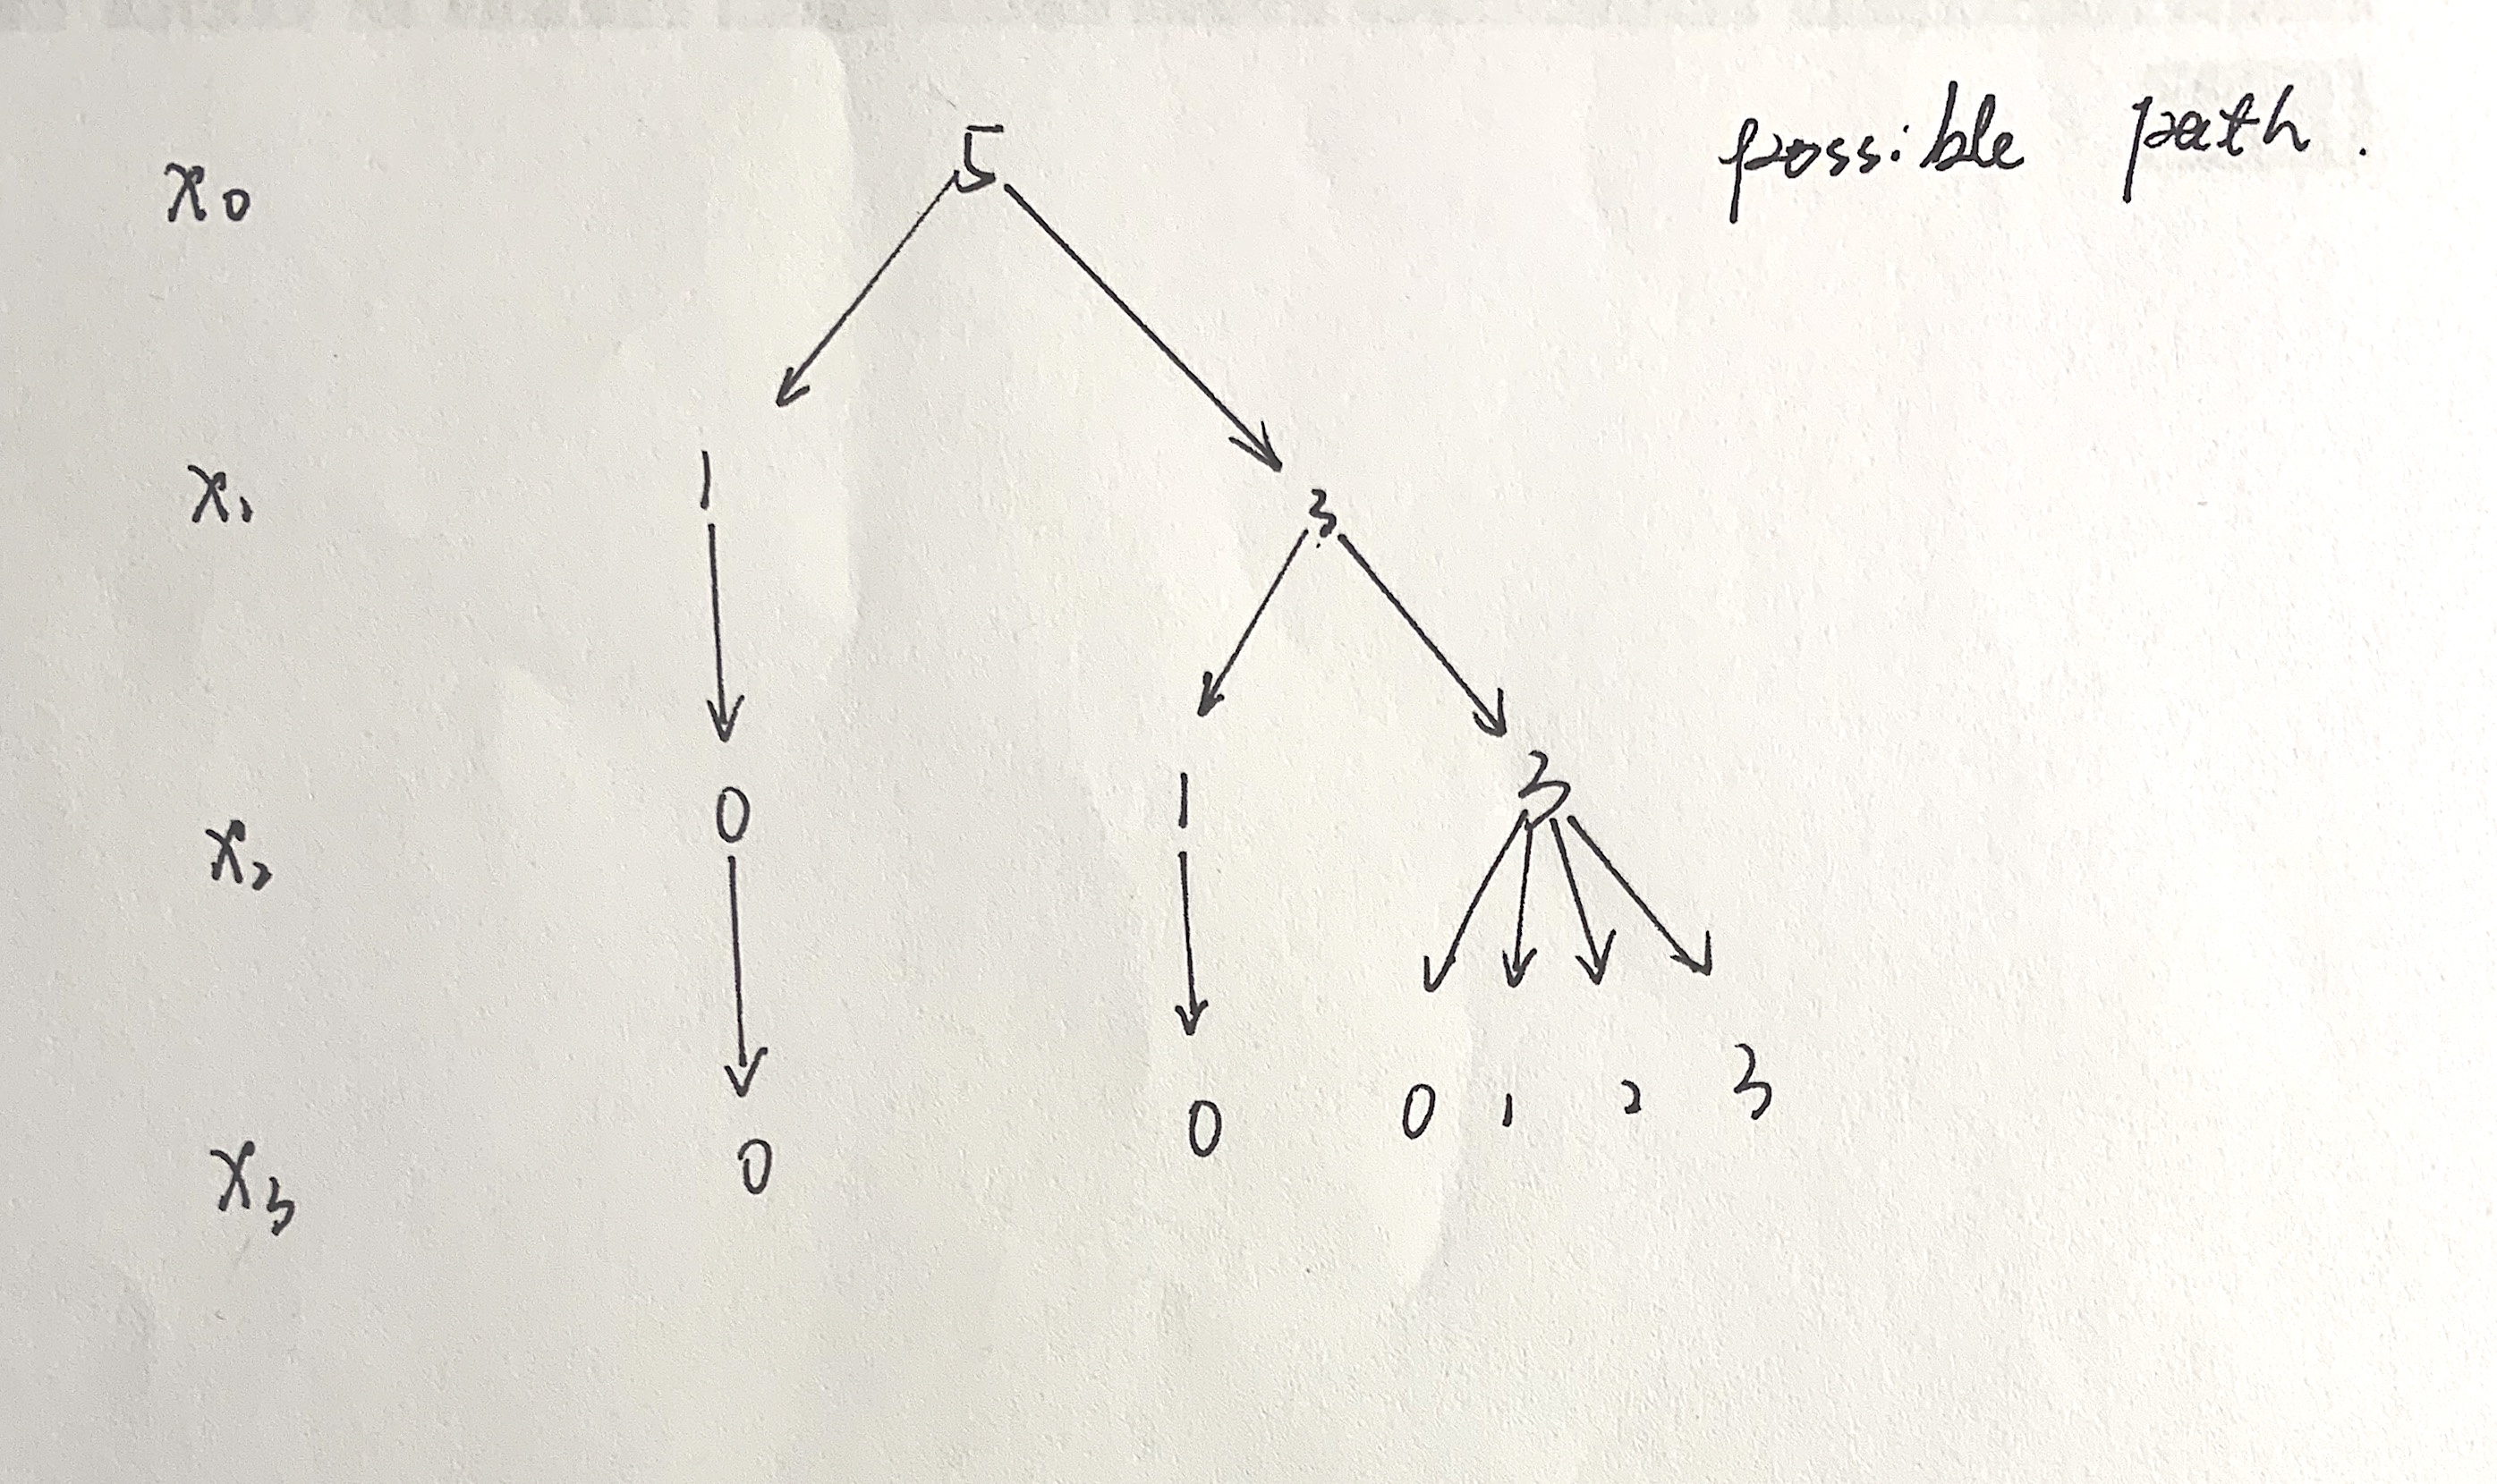
\includegraphics[width = .8\textwidth]{dp7.jpg}
  \caption{}
  \label{dp7}
\end{figure} 

The expected optimal cost $J^{*} = 43.25$, the optimal policy is $u_0 = -3$, $u_1(1) = -1$,  $u_1(3) = -2$,
$u_2(0) = 0$, $u_2(1) = -1$, $u_2(3) = -2\ or\ -1$. 

Correction: (*Again mistakes were made when $x_0 = 5 $ applying control ($u_0 = -3$) the cost is 43.25 and when $x_1 =2$ applying $u_1 = -2$ the cost is minimum 8)
\end{itemize}



\section*{Exercise 2 [Controllability]}

\begin{itemize}
  \item When $u_n = 0$, the systems of form $x_{n+1} = Ax_n$ are stable if.f all eigenvalues of A have magnitude strictly less than unity.
  
  for a) and b) the eigenvalues of A are $(1.61803399, -0.61803399,  1.5)$;

  for c) the eigenvalues of A are $(0.5, -0.5,  0.5)$; 

  for d) the eigenvalues of A are $(0.70380158$,  $0.24007567$, $-0.44387725)$.

  Therefore c) and d) are stable systems when $u_n = 0$.
  \item The systems of form $x_{n+1} = Ax_n+Bu_n$ are controllable if.f the matrix 
  \begin{equation}
  S = [B \ AB\  A^2B\ \cdots\  A^{k-1}B] 
  \end{equation}
  is full row rank (where k is the size of vector $x_n$)
  
  for a) 
  \begin{equation}
  S = \left[\begin{matrix} & 0 & 1 & 1 &\\ & 0 & 0 & 0 &\\ & 1 & 0 & 1 &\end{matrix}\right] \nonumber
  \end{equation}

  for b) 
  \begin{equation}
  S = \left[\begin{matrix} & 0 & 1 & 1 &\\ & 1 & 1.5 & 2.25 &\\ & 1 & 0 & 1 &\end{matrix}\right] \nonumber
  \end{equation}
  for c)
  \begin{equation}
  S = \left[\begin{matrix} & 1 & 1 & 0.75 &\\ & 0 & -1 & 0 &\\ & 1 & 0.5 & 0.25 &\end{matrix}\right] \nonumber
  \end{equation}
  for d)
  \begin{equation}
  S = \left[\begin{matrix} & 0 & 0.5 & 0 &\\ & 1 & -0.5 & 0.25 &\\ & 0 & 0 & -0.05 &\end{matrix}\right] \nonumber
  \end{equation}

  Therefore a) is not controllable b), c), d) are controllable.

  \item If a system is controllable, then the LQR optimal control makes the system stable, so for b), c) and d) we can find a
  law $u_n$ to stablize the systems.
\end{itemize}


\section*{Exercise 3 [Linear Quadratic Regulators]}

As answered in Jupyter notebook file $Linear\ Quadratic\ Regulators.ipynb$


\section*{Exercise 4 [Cart-Pole Model]}

As answered in Jupyter notebook file $Cart-Pole\ Model.ipynb$


\section*{Exercise 5 [Direct Transcription]}

As answered in Jupyter notebook file $Direct\ Transcription\ Methods.ipynb$


\end{document}
